\section{Mixnät}
\begin{frame}
\frametitle{Innehåll}
\tableofcontents[currentsection]
\end{frame}

\begin{frame}{Mixnät}

\begin{columns}
    \begin{column}{0.4\textwidth}
        \begin{itemize}
        	\item Mixnät blandar
        	\item Hur går detta till?
        \end{itemize}
    \end{column}
	\begin{column}{0.6\textwidth}
    	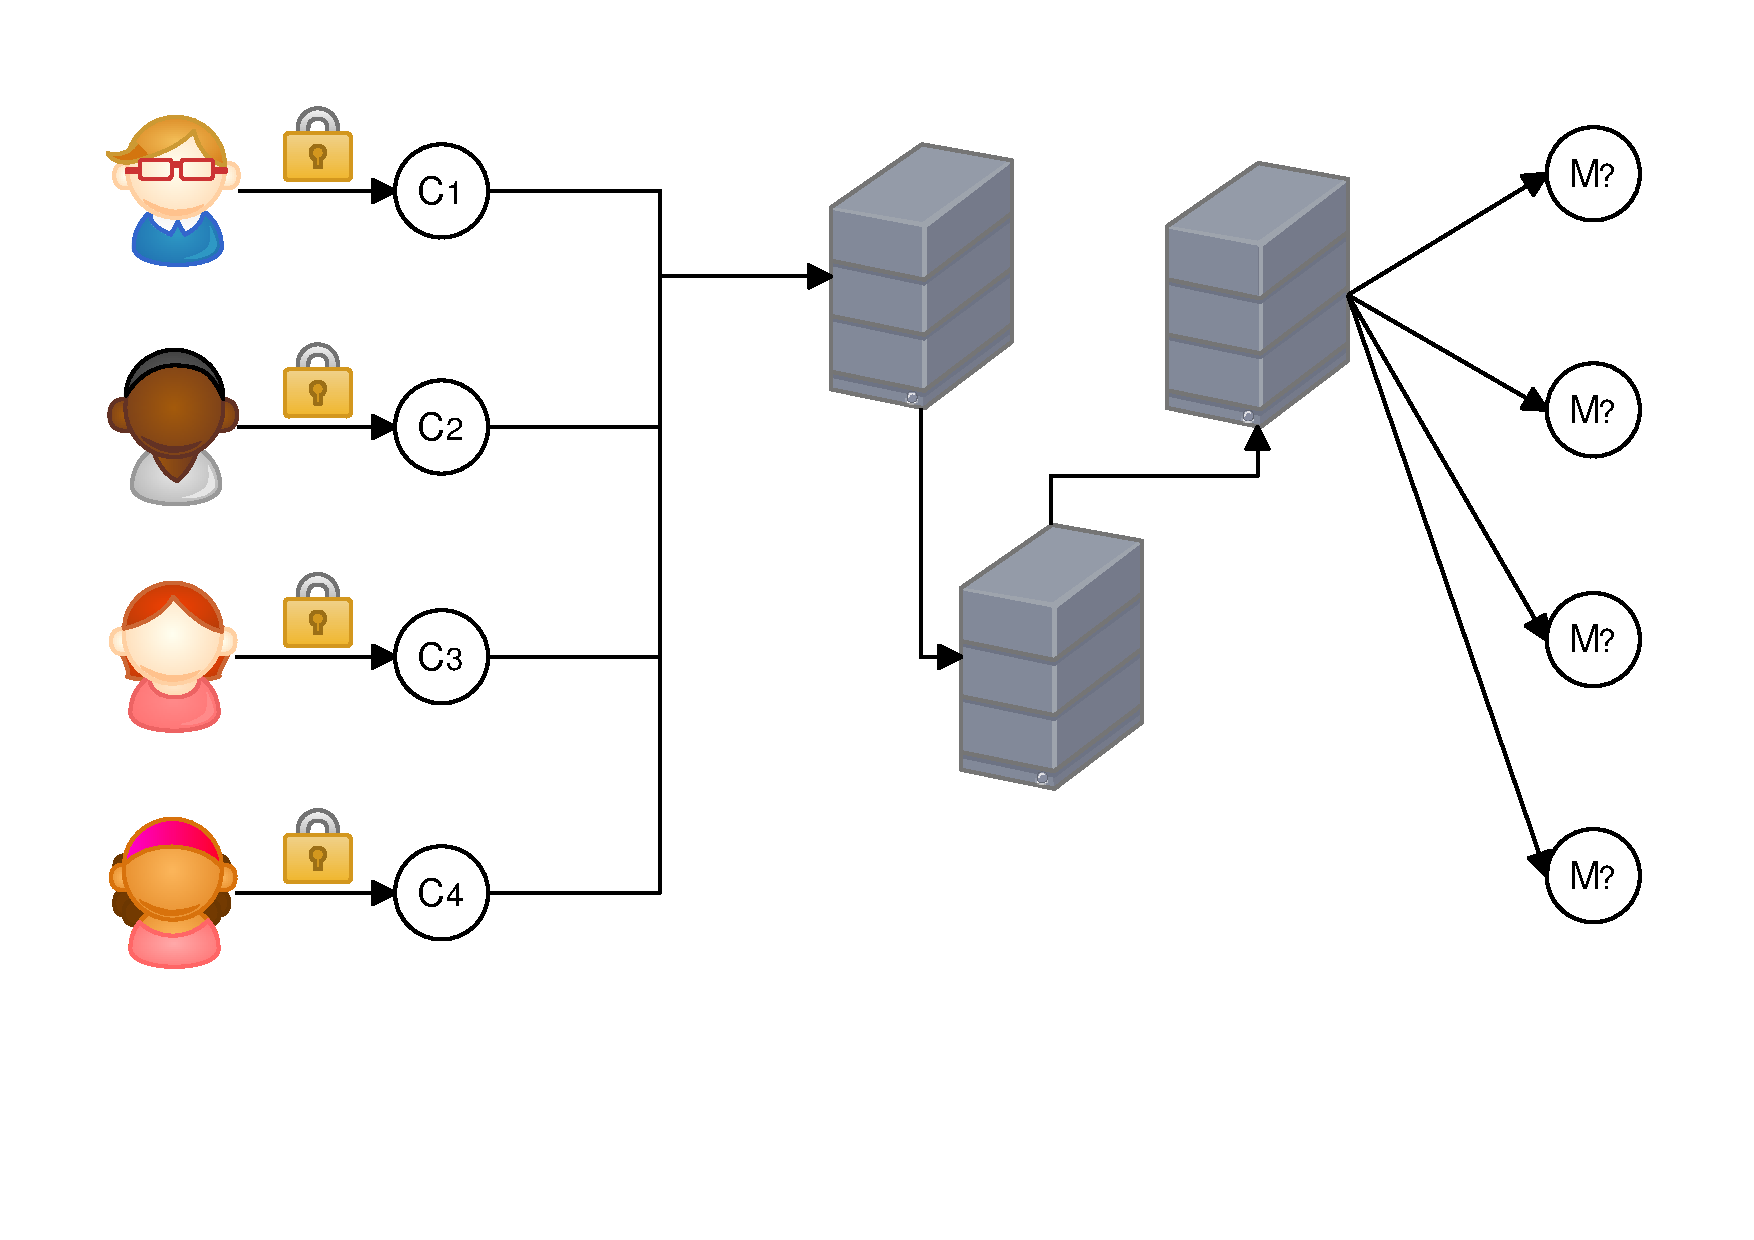
\includegraphics[width=\textwidth]{images/mix1.pdf}
	\end{column}
\end{columns}

\end{frame}

\begin{frame}{Hur fungerar varje server?}

\begin{columns}
    \begin{column}{0.4\textwidth}
        \begin{itemize}
        	\item Indata: kryptotexter
        	\item Kryptera om
        	\item Blanda
        	\item Mata ut
        \end{itemize}
    \end{column}
	\begin{column}{0.6\textwidth}
    	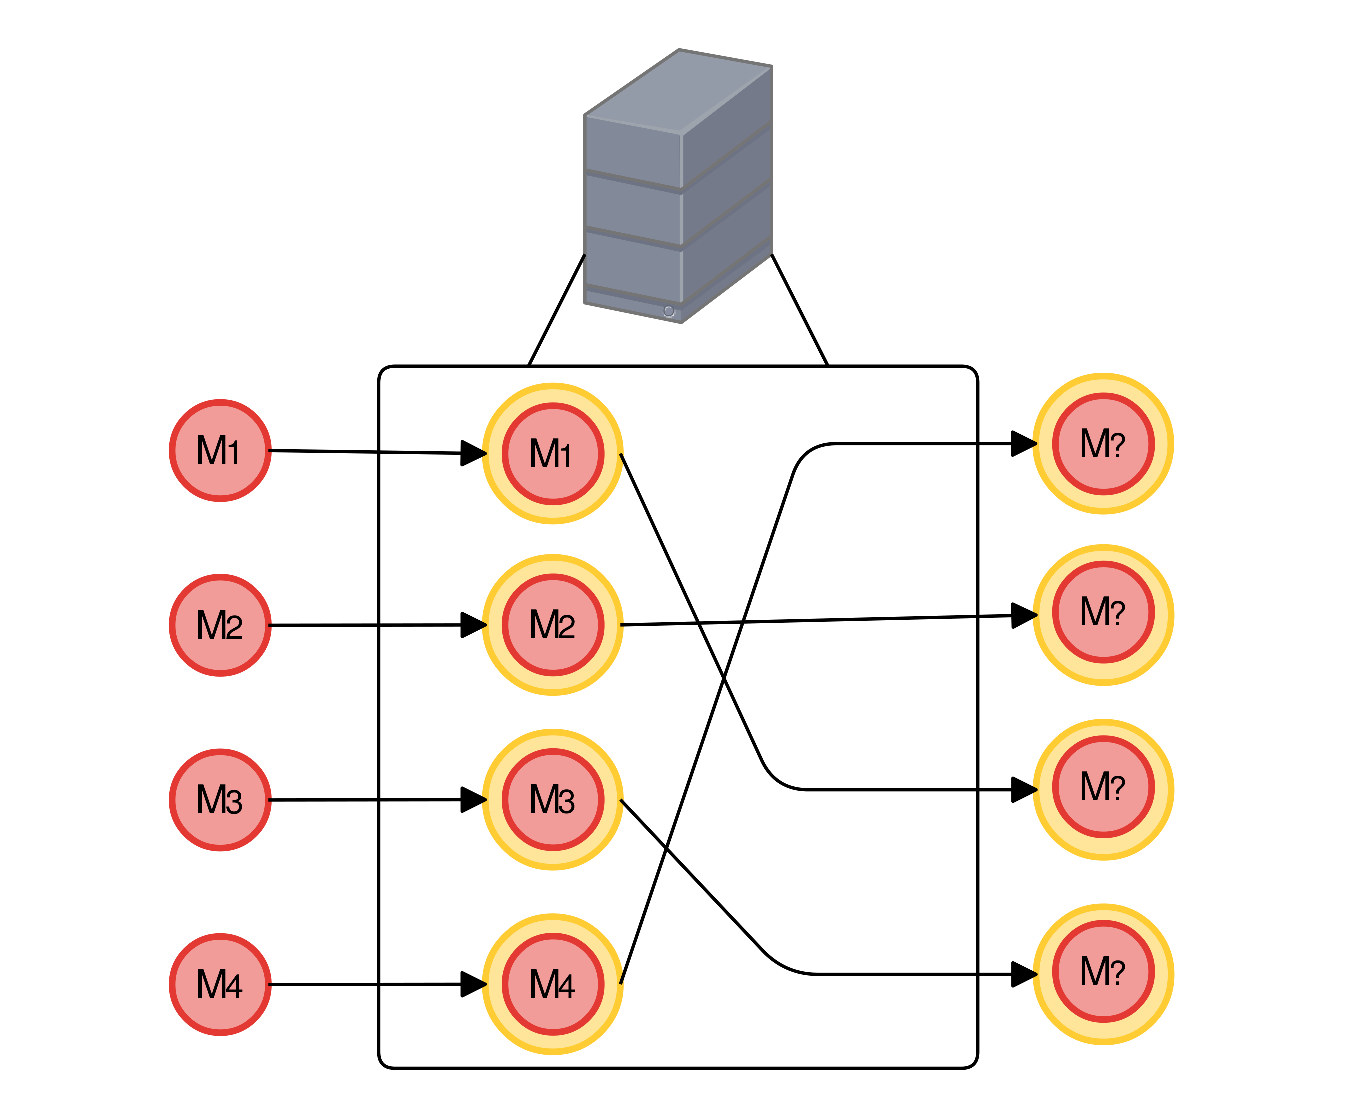
\includegraphics[width=\textwidth]{images/mix4.pdf}
	\end{column}
\end{columns}


\end{frame}

\begin{frame}{Hur kan vi verifiera att det blir rätt?}

\begin{columns}
    \begin{column}{0.4\textwidth}
        \begin{itemize}
        	\item Verifiering
        	\item Zero-knowledge
        	\item Extra data
        \end{itemize}
    \end{column}
	\begin{column}{0.6\textwidth}
    	\only<1>{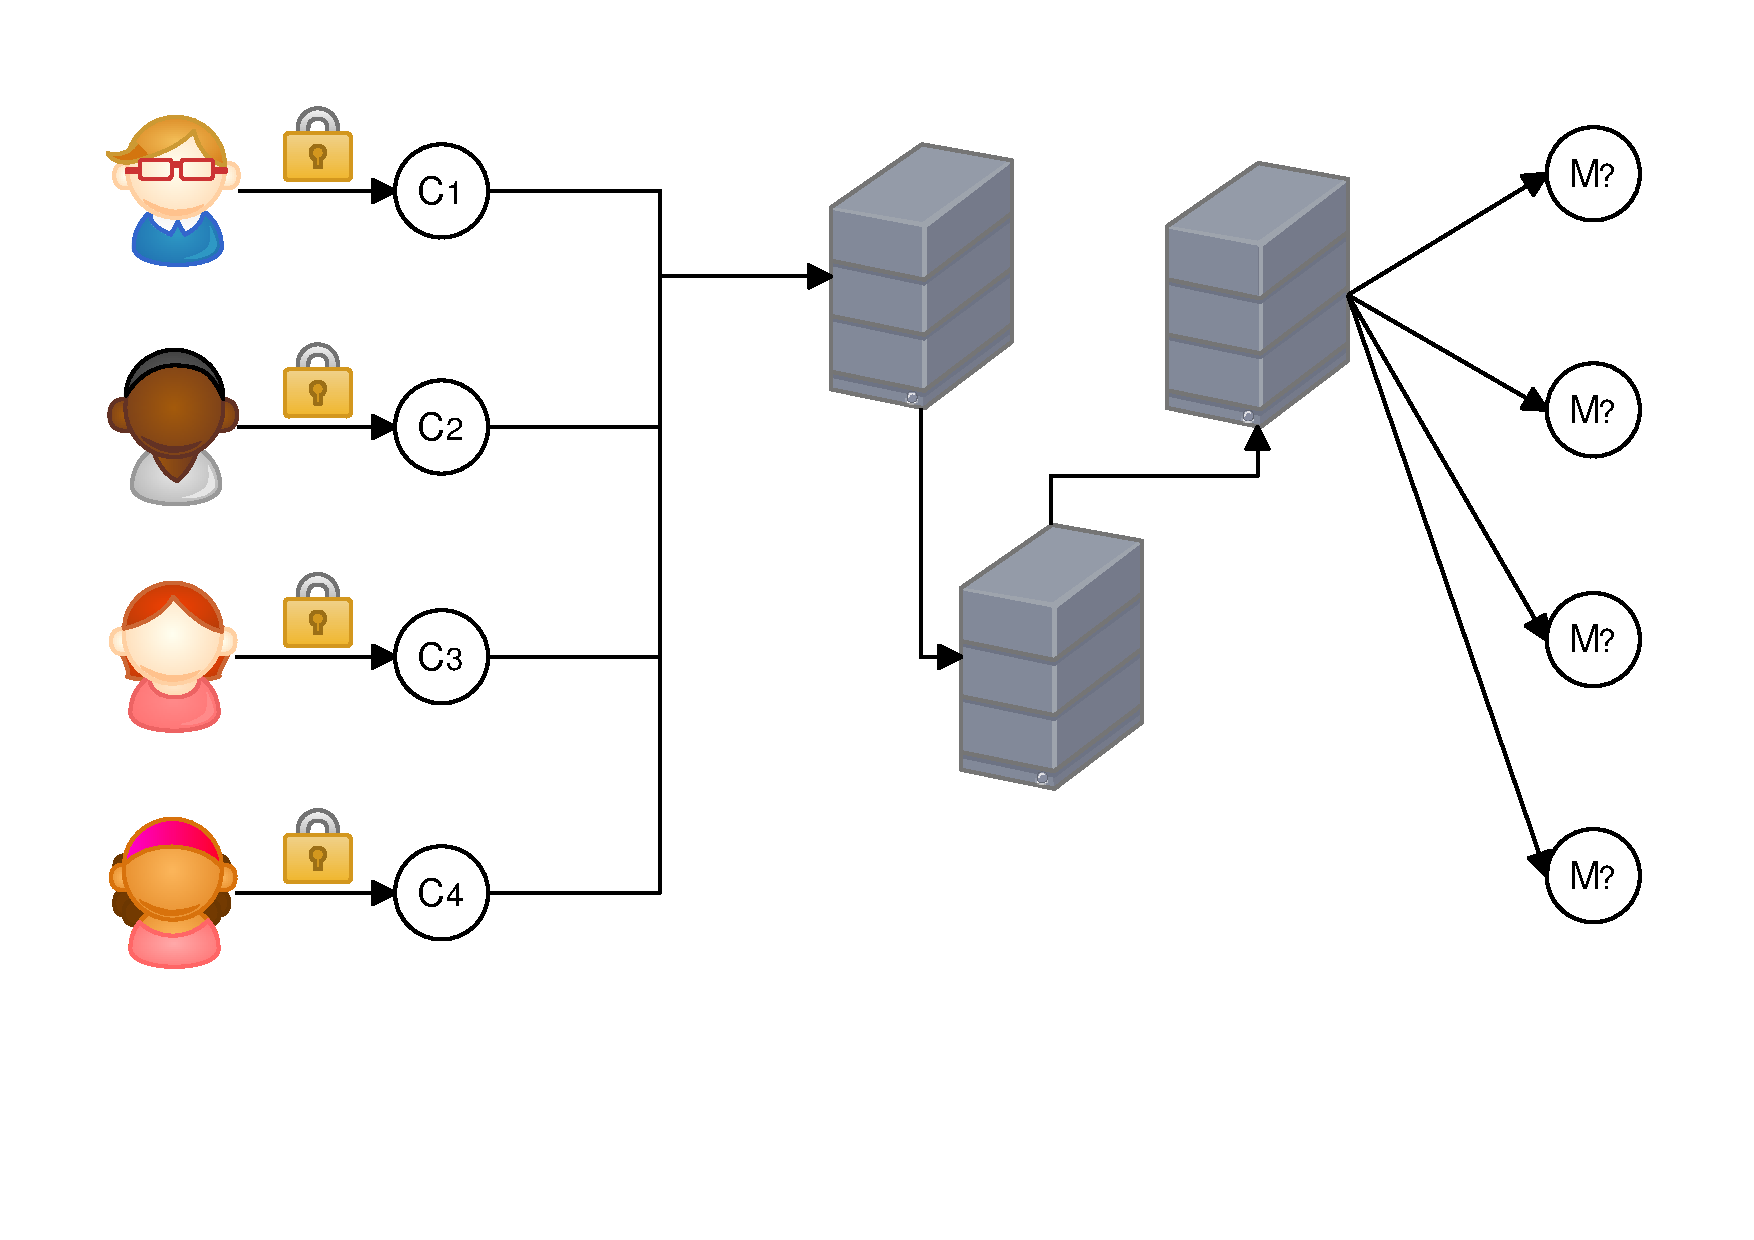
\includegraphics[width=\textwidth]{images/mix1.pdf}}
    	\only<2>{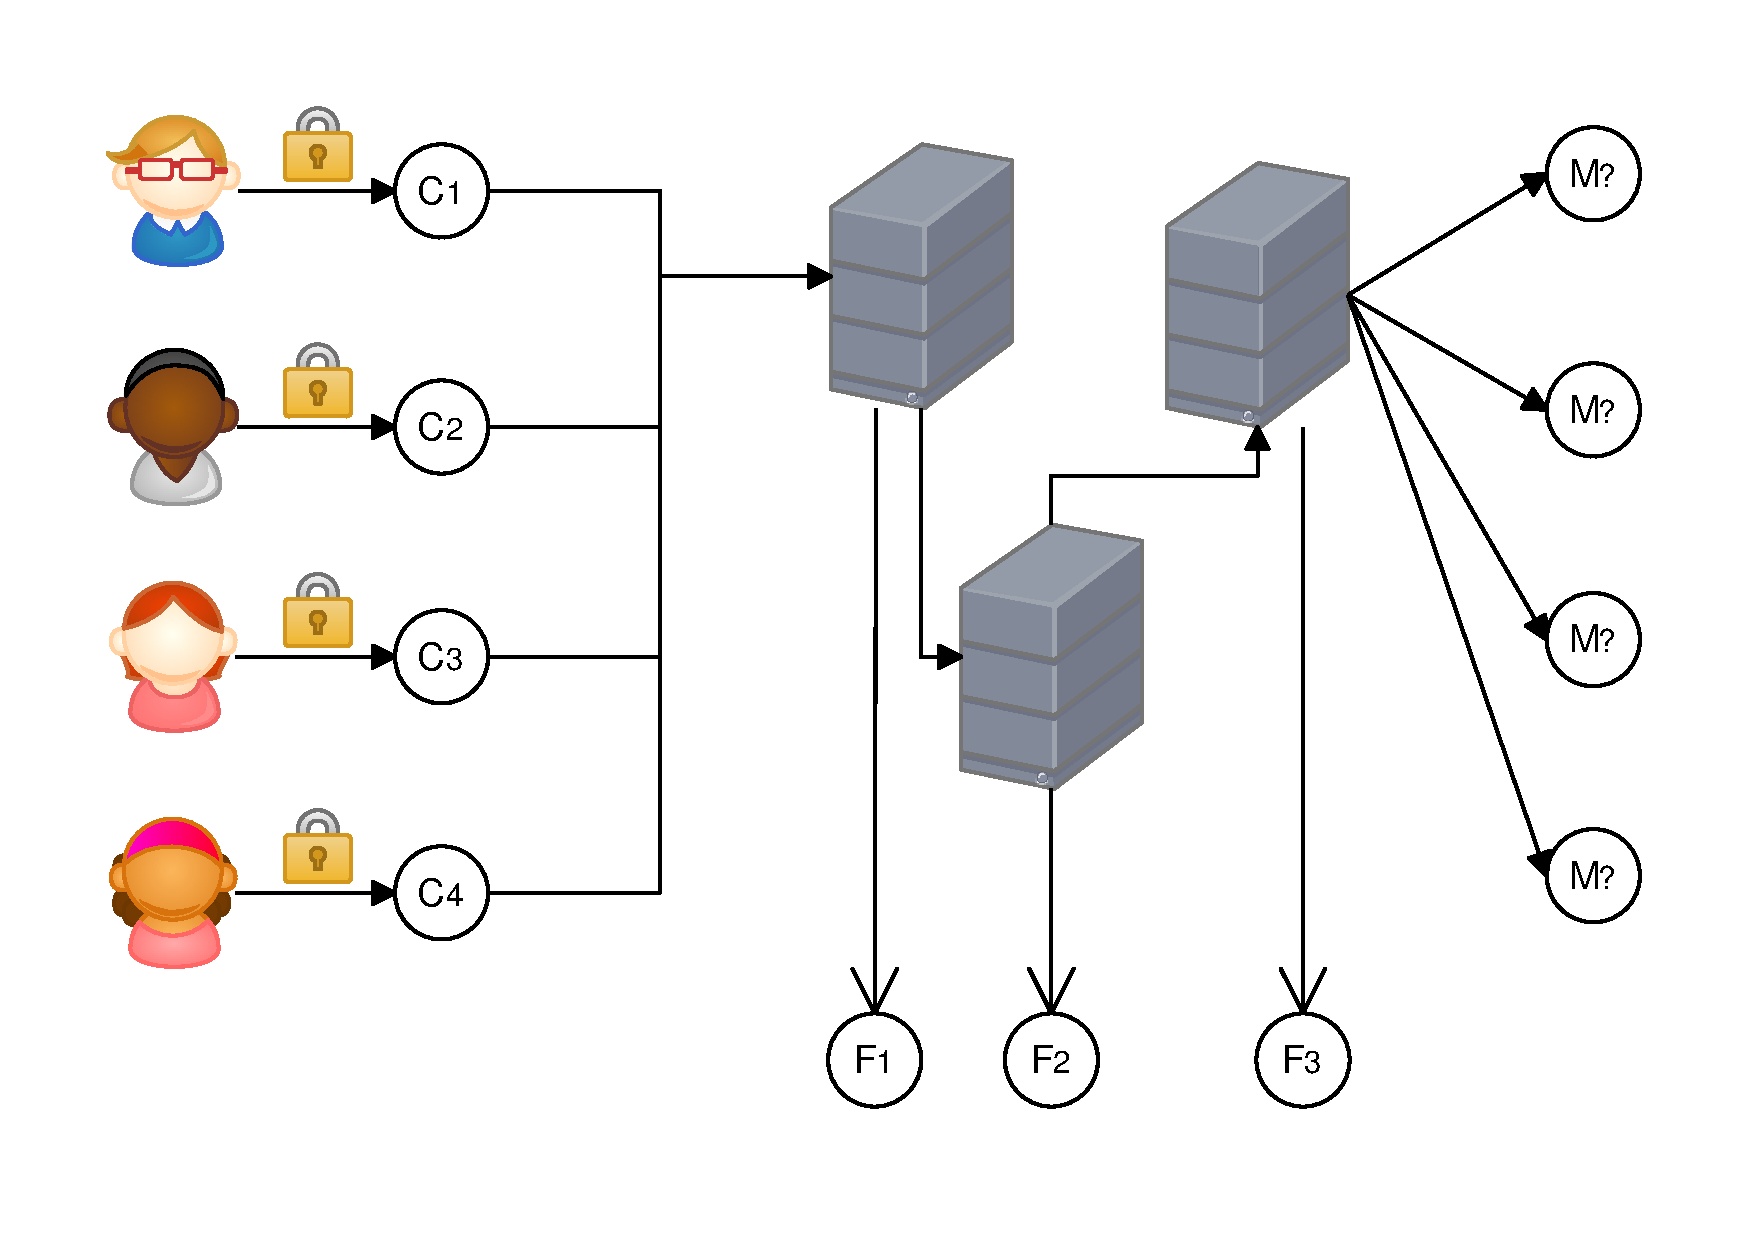
\includegraphics[width=\textwidth]{images/mix2.pdf}}
	\end{column}
\end{columns}

\end{frame}

\begin{frame}{Verifieraren analyserar körningen}

\begin{center}
  \makebox[\textwidth]{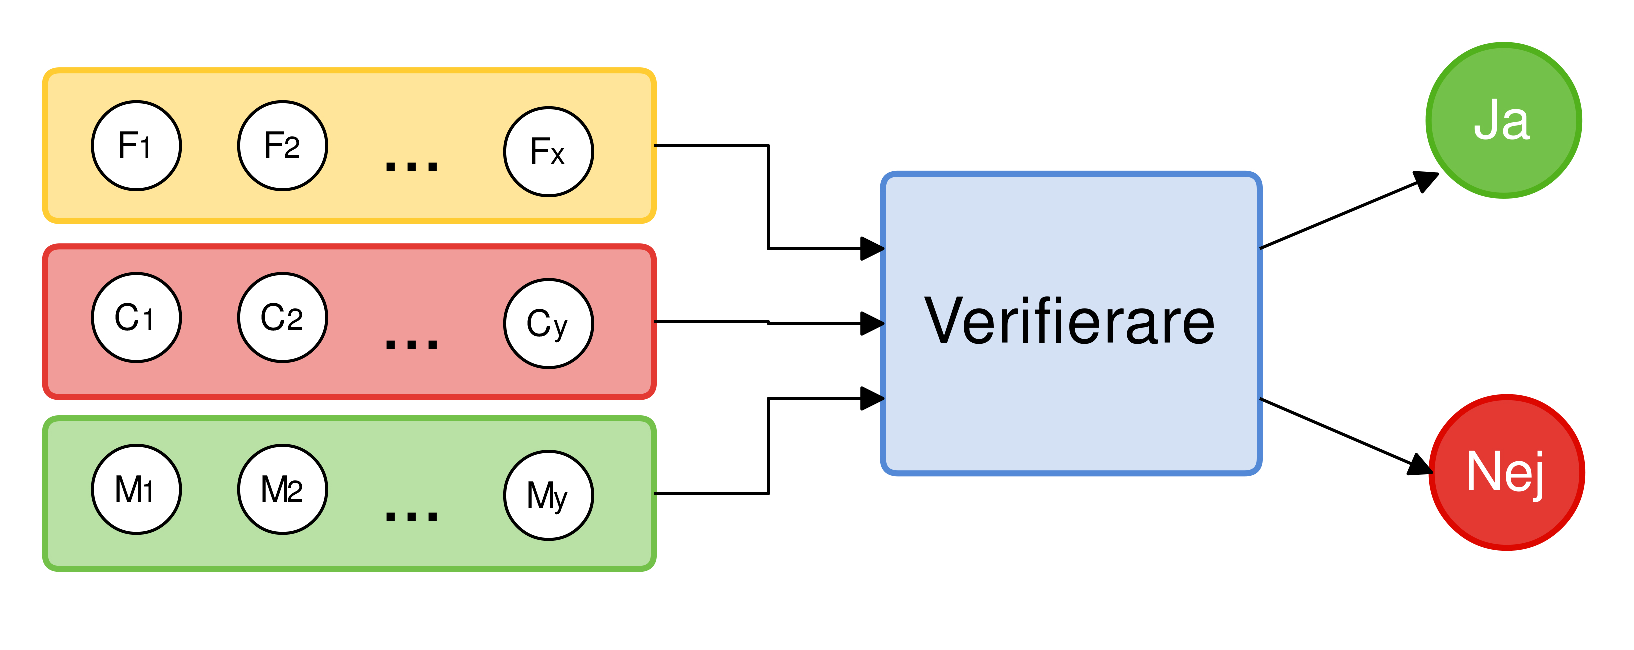
\includegraphics[width=\textwidth]{images/mix3.pdf}}
\end{center}

\begin{itemize}
\item Vi får reda på om allt gått rätt till
\item Fortfarande inte möjligt att veta vems röst som är vem
\end{itemize}

\end{frame}

\section{Verificatum}
\begin{frame}
\frametitle{Innehåll}
\tableofcontents[currentsection]
\end{frame}

\begin{frame}{Vad är Verifactum?}

\begin{itemize}
\item Implementation av mixnät
\item Verifierbart
\item Vem som helst ska kunna verifiera
\item Specifikationsdokument
\begin{itemize}
	\item[-] Är det korrekt?
	\item[-] Är det användbart?
\end{itemize}
\end{itemize}

\end{frame}
